A clear understanding of the background of this project comes from appreciating three different key aspects: Lakehouse development, Apache Spark relevance and flows, and Python as an emergent language.

Lakehouse is a term coined by Databricks in 2020 \cite{WhatLakehouse2020}, to define a new design standard that was emerging in the industry that combined the capability of data lakes in storing and managing unstructured data, with the \gls{ACID} properties typical of Data warehouses.
Data warehouses became a dominant standard in the '90s and early 2000s \cite{chaudhuriOverviewDataWarehousing1997}, enabling companies to generate \gls{BI} insights, managing different structured data sources. The problems related to this architecture were highlighted in the 2010s when the need to manage large quantities of unstructured data rose \cite{ederUnstructuredData802008}. 
So Data lakes became the pool where all data could be stored, on top of which a more complex architecture could be built, consisting of data warehouses for \gls{BI} and \gls{ML} pipelines.
This architecture, while more suitable for unstructured data, introduces many complexities and costs, related to the need of having replicated data (data lake and data warehouse), and several \gls{ELT} and \gls{ETL} computations.
Lakehouse systems solved the problems of Data lakes by implementing data management and performance features on top of open data formats such as Parquet \cite{DremelMadeSimple}. Three key technologies enabled this paradigm: (i) a metadata layer for data lakes, tracking which files are part of different tables, (ii) a new query engine design, providing optimizations such as RAM/SSD caching, and (iii) an accessible \gls{API} access for \gls{ML} and \gls{AI} applications. This architecture design was first open-sourced with Apache Hudi in 2017 \cite{rajaperumalUberEngineeringIncremental2017} and then Delta Lake in 2020 \cite{armbrustDeltaLakeHighperformance2020}.

Spark is a distributed computing framework used to support large-scale data-intensive applications \cite{zaharia2010spark}. Spark builds from the roots of MapReduce and its variants. MapReduce is a distributed programming model first designed by Google that enables the management of large datasets \cite{dean2004mapreduce}. The paradigm was later implemented as an open-source project by Yahoo! engineers under the name of Hadoop MapReduce \cite{borthakurHadoopDistributedFile2005}. Spark significantly improved the performance of Hadoop MapReduce (10 times better in its first iteration) \cite{zaharia2010spark} thanks to its use of \glspl{RDD} \cite{Zaharia:EECS-2011-82}. \glspl{RDD} is a distributed memory abstraction that enables a lazy in-memory computation that is tracked through the use of lineage graphs, ultimately increasing fault tolerance \cite{Zaharia:EECS-2011-82}. This means that Spark avoids going back and forth between storage disks to store the computation results, as represented in Figure \ref{fig:MapReducevsSpark}.

\begin{figure}[!ht]
    \begin{center}
      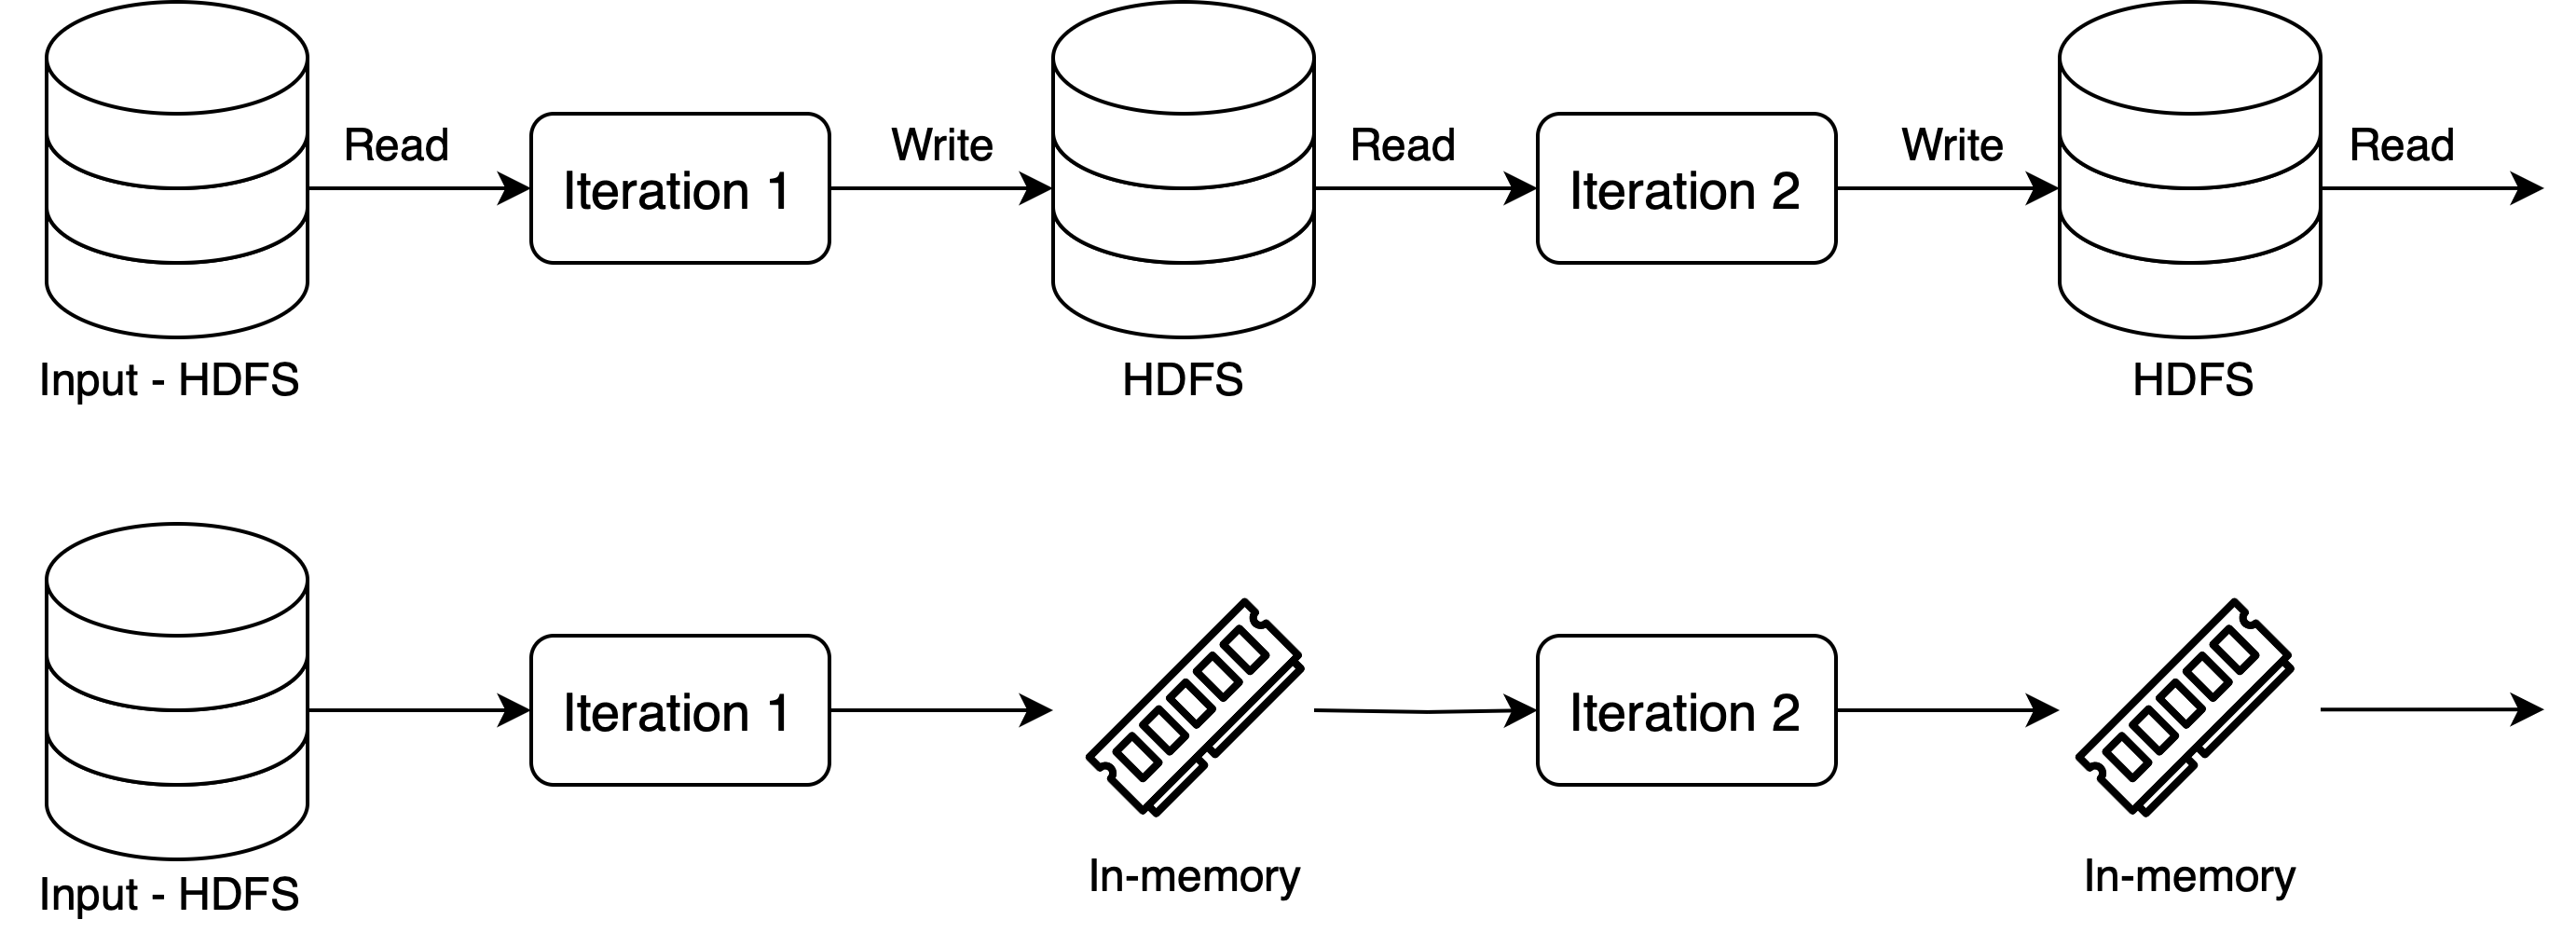
\includegraphics[width=\textwidth]{figures/1-introduction/Spark_MapReduce.png}
    \end{center}
    \caption{Hadoop MapReduce and Apache Spark execution differences}
    \label{fig:MapReducevsSpark}
\end{figure}


Spark, which is open-sourced under the Apache foundation as Apache Spark \cite{ApacheSparkUnified} (from now on simply Spark), has seen widespread success and adoption in various applications, becoming the de-facto data-intensive computing platform for the distributed computing world. While Spark is often used as a comprehensive solution \cite{zahariaApacheSparkUnified2016}, different solutions might be better suited for a specific scenario. An example of this is the case of Apache Flink \cite{carboneApacheFlinkStream}, designed for real-time data streams, which prevails over Spark where low latency real-time analytics are required. Similarly, Spark might not be the best tool for lower-scale applications where the high-scaling capabilities of Spark may not be required. This is the case of DuckDB \cite{raasveldtDuckDBEmbeddableAnalytical2019} and Polars \cite{vinkWroteOneFastest2021}, that by focusing on low scale (10GB-100GB) provide a fast \gls{OLAP} embedded database and DataFrame management system respectively offering an overall faster computation compared to starting a Spark cluster for to perform the same operations. This shows the possibility for improvements and new applications that substitute the current Spark-based systems in specific applications such as real-time data streaming or small-scale computation. In this project, the latter application is going to be explored.

Python can be considered the primary programming language among data scientists \cite{Python_CS-R9526}. Many first adopted Python thanks to its focus on ease of use, high abstraction level, and readability. This helped create a fast-growing community behind the project, which led to the development of many libraries and \glspl{API}. So now, more than 30 years after its creation, it has become the de-facto standard for data science thanks to many daily used Python libraries such as TensorFlow, NumPy, SciPy, Pandas, PyTorch, Keras and many others.

Python is also considered to be the most popular programming language, according to the number of results by search query (\textit{+"<language> programming"}) in 25 different search engines \cite{TIOBEIndexa}. This is computed yearly in the TIOBE Index \cite{TIOBEIndex}. Looking at the 2024 list, it can be noted that Python has a rating of 15.16\%, followed by C which has a rating of 10.97\%. The index also shows the trends of the last years, clearly displaying the rise of Python over historically very popular languages such as C and JAVA, which were both outranked by Python between 2021 and 2022. This shows the importance of offering Python \glspl{API} for programmers and data scientists in particular to increase the engagement and possibilities of a framework.